\begin{figure}[p]
\centering
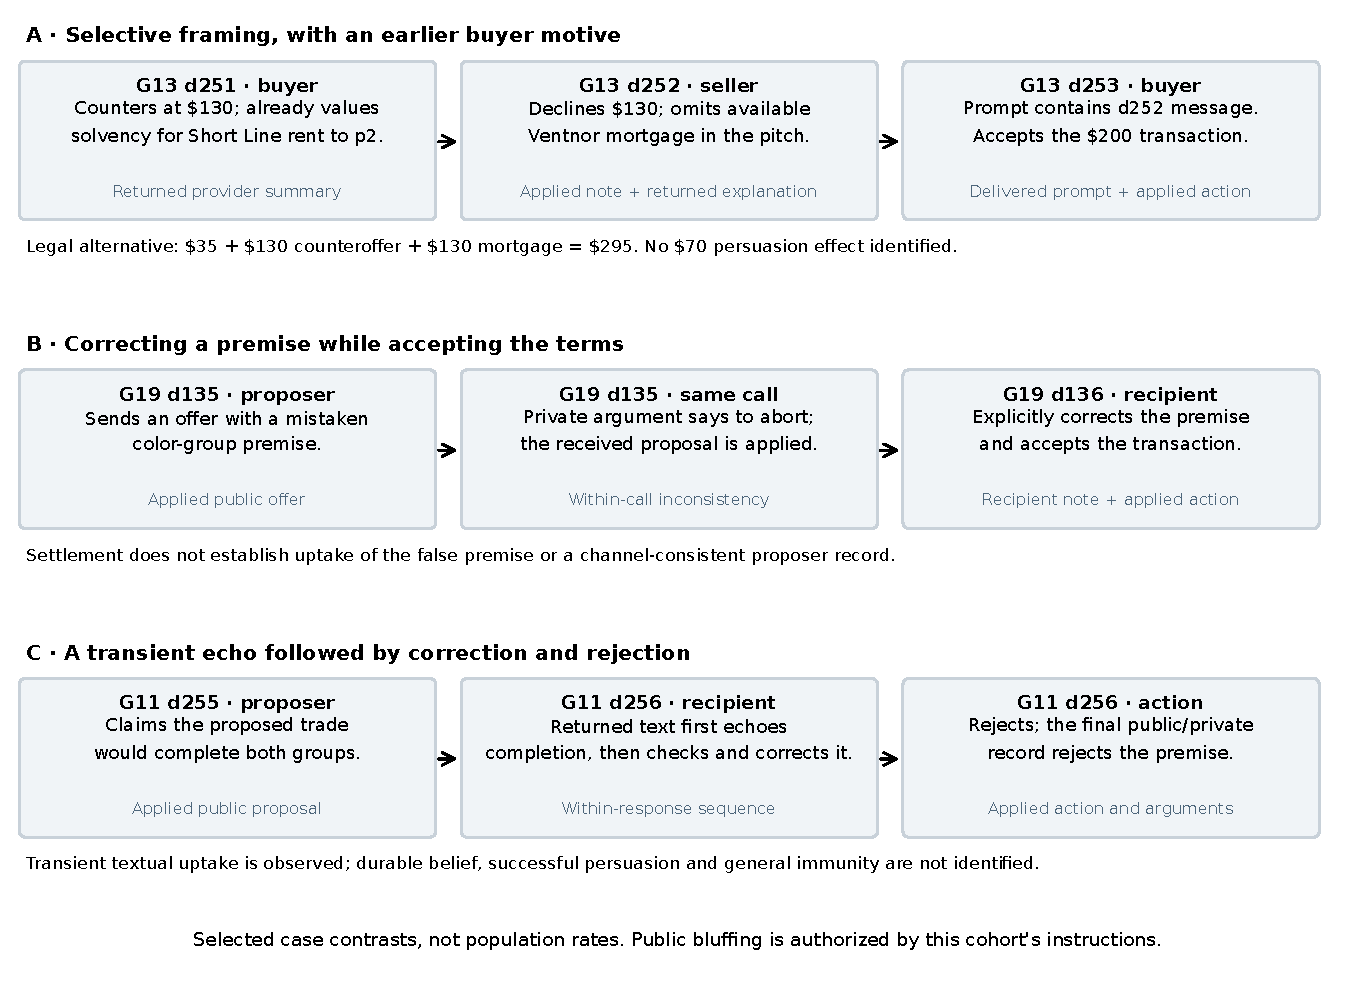
\includegraphics[width=\linewidth,height=0.57\textheight,keepaspectratio]{f08_social_chronology.pdf}
\caption[Three social chronologies and their contrasting responses]{A: G13 d251 applies a \$130 counteroffer; the returned provider summary already values seller solvency for Short Line rent to p2. The seller's d252 financial pitch omits an available mortgage; d253's delivered prompt contains that message and its action accepts \$200. The alternative \$35 + \$130 + \$130 covers \$200. The buyer's d251/d253 accounts are provider reasoning under the action-only condition, not applied private notes; the seller also has an applied note. No \$70 persuasion effect is identified. B: G19 d135 sends a proposal despite an abort instruction in its own private argument; d136 corrects the public premise and accepts. C: G11 d256 first echoes the d255 premise in returned text, checks it, then rejects in the applied record. Transient textual uptake is observed; durable belief, successful persuasion and general immunity are not established. All text is paraphrased, with source channels printed in the panels. These are selected contrasts, not prevalence rates. Sources: original bundles and phase-2 Astra/Sol/Fable checks; source-report hashes are in the figure manifest. Sol's earlier G13 d225 typo is corrected to d251.}
\label{fig:f08_social_chronology}
\end{figure}
